\chapter{Lexique-grammaire}
\label{chap-lexicon-grammar}
\index{Lexique-grammaire}
Les tables de lexique-grammaire sont un moyen compact de représenter les propriétés
syntaxiques des éléments d’une langue. Il est possible de construire automatiquement des
grammaires locales à partir de ces tables, grâce à un mécanisme de graphes paramétrés.


\bigskip
\noindent La première partie de ce chapitre présente le formalisme de ces tables. La seconde partie
décrit les graphes paramétrés et le mécanisme de génération automatique de graphes à partir d’une
table de lexique-grammaire.



\section{Les tables de lexique-grammaire}
\index{Lexique-grammaire!table}\index{Matrices}
Le lexique-grammaire est une méthodologie qui a été développée par Maurice Gross et
son équipe du LADL\index{LADL} (\cite{L}, \cite{BGL}, \cite{methodes-en-syntaxe}, \cite{GL},
\cite{gross1994}, \cite{gross1994b}, \cite{gross1991}, \cite{gross1986}, 
\cite{gross1984}, \cite{gross1984b}, \cite{gross1983}, \cite{gross1982}, 
\cite{gross1978}, \cite{leclere2005}, \cite{salkoff2004})
sur le principe suivant : chaque verbe a des propriétés syntaxiques quasiment uniques.
De ce fait, ces propriétés doivent être systématiquement décrites, car il est impossible de prévoir
le comportement précis d’un verbe. Ces descriptions systématiques sont représentées au moyen de
matrices où les lignes correspondent aux verbes, et les colonnes aux propriétés syntaxiques. Les
propriétés considérées sont des propriétés formelles telles que le nombre et la nature des
compléments admis par le verbe et les différentes transformations que ce verbe peut subir
(passivation, nominalisation, extraposition, etc.).
Les matrices, plus souvent appelées tables, sont binaires : un signe  \verb$+$ apparaît à
l’intersection d’une ligne et d’une colonne d’une propriété si le verbe vérifie la propriété,
un signe \verb+-+ sinon.\index{Propriétés syntaxiques} Pour plus d'information consulter
\url{http://infolingu.univ-mlv.fr}, où des tables du lexique-grammaire sont librement
téléchargeables.

\bigskip
\noindent Ce type de description a aussi été utilisé pour les adjectifs 
(\cite{these-annie}), les noms prédicatifs (\cite{les-nominalisations},
\cite{les-predicats-nominaux}, \cite{giry1978}, \cite{gross1976},
\cite{ranchhod2001}), adverbes (\cite{syntaxe-de-ladverbe},
\cite{grammaire-des-adverbes}), ou les expressions figées, dans de nombreuses langues
(\cite{lexique-grammaire-allemand2}, \cite{lexique-grammaire-italien2},
\cite{lexique-grammaire-italien}, \cite{lexique-grammaire-coreen2},
\cite{lexique-grammaire-coreen}, \cite{lexique-grammaire-malgache},
\cite{lexique-grammaire-espagnol}, \cite{lexique-grammaire-allemand},
\cite{lexique-grammaire-hongrois}, \cite{ranchhod1996}, \cite{ranchhod1991},
\cite{gross1986b}).

\bigskip
\noindent La figure~\ref{fig-table-32NM} montre un exemple de table de lexique-grammaire. Cette
table concerne les verbes admettant un complément numérique.


\begin{figure}[!ht]
\begin{center}
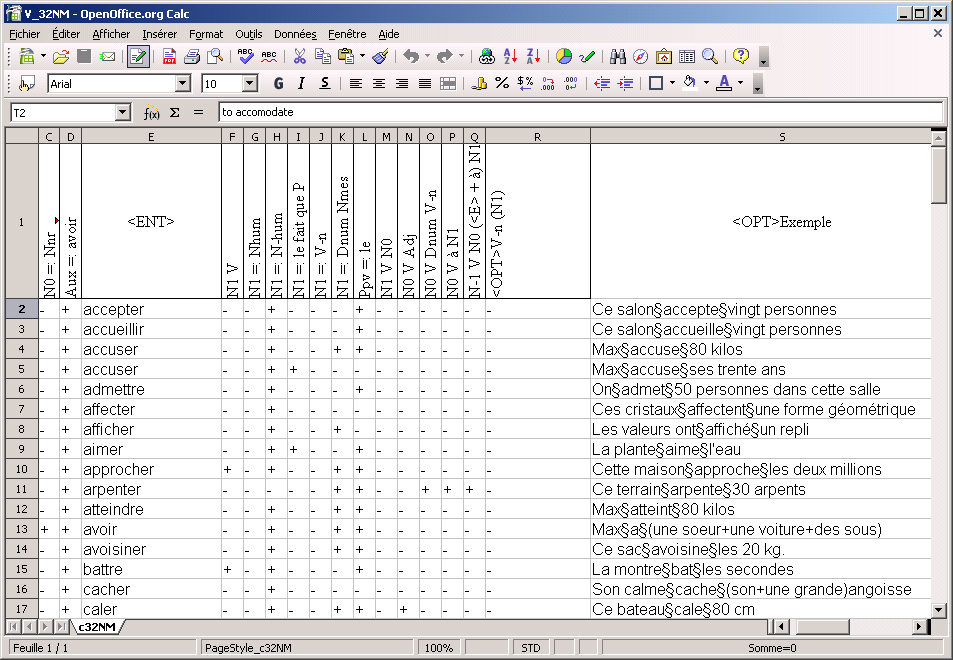
\includegraphics[width=15cm]{resources/img/fig8-1.png}
\caption{Table de lexique-grammaire 32NM\label{fig-table-32NM}}
\end{center}
\end{figure}

\section{Conversion d’une table en graphes}
\subsection{Principe des graphes paramétrés}
\index{Graphe!paramétré}
La conversion d’une table en graphes s’effectue au moyen du mécanisme des graphes
paramétrés. Le principe est le suivant : on construit un graphe qui décrit des constructions
possibles. Ce graphe fait référence aux colonnes de la table grâce à des variables. On génère
ensuite, pour chaque ligne de la table, une copie de ce graphe dans laquelle les variables
sont remplacées en fonction du contenu des cellules situées à l’intersection des colonnes
correspondantes et de la ligne traitée. Si une cellule de la table contient le signe
 \verb$+$ la variable correspondante est remplacée par \verb+<E>+. Si la cellule contient le signe
\verb+-+,la boîte contenant la variable correspondante est supprimée, ce qui détruit du même coup
les chemins passant par cette boîte. Dans tous les autres cas, la variable est remplacée par le
contenu de la cellule.



\subsection{Format de la table}
Les tables de lexique-grammaire sont généralement codées à l’aide d’un tableur comme
OpenOffice.org Calc (\cite{OpenOffice}). Pour pouvoir être utilisées par Unitex, les tables doivent
être codées en texte Unicode selon la convention suivante : les colonnes doivent être séparées
par des tabulations et les lignes par des retours à la ligne.


\bigskip
\noindent Pour convertir une table avec OpenOffice.org Calc, sauvegardez-la au format texte
(extension \verb$.csv$). Le programme vous propose ensuite de paramétrer la sauvegarde au moyen
d’une fenêtre comme celle de la figure~\ref{fig-csv-export}. Choisissez le codage "Unicode",
sélectionnez la tabulation comme séparateur de colonnes, et ne précisez pas de délimiteur de texte.

\begin{figure}[!ht]
\begin{center}
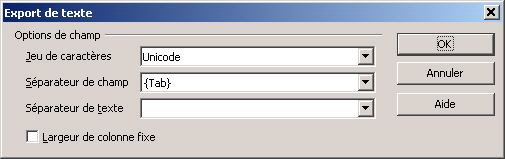
\includegraphics[width=12cm]{resources/img/fig8-2.png}
\caption{Configuration de la sauvegarde d’une table avec OpenOffice.org Calc\label{fig-csv-export}}
\end{center}
\end{figure}

\bigskip
\noindent Lors de la génération des graphes, Unitex saute la première ligne, considérée comme
donnant les en-têtes des colonnes. Vous devez donc vous assurer que les en-têtes des colonnes
occupent exactement une ligne. S’il n’y a pas de ligne d’en-tête, la première ligne de
la table sera ignorée, et s’il y a plusieurs lignes d’en-tête, elles seront interprétées à partir de
la deuxième comme des lignes de la table.



\subsection{Les graphes paramétrés}
Les graphes paramétrés sont des graphes dans lesquels apparaissent des variables fai-
sant référence aux colonnes d’une table de lexique-grammaire. On utilise généralement
ce mécanisme avec des graphes syntaxiques, mais rien n’empêcherait de construire des
graphes paramétrés de flexion, de prétraitement ou de normalisation.


\index{Variable!dans un graphe paramétré}
\bigskip
\noindent Les variables qui font référence aux colonnes sont formées du caractère \verb+@+
\index{\verbc{"@}} suivi d’un nom de colonne en lettres majuscules (les colonnes sont numérotées
en partant de \verb+A+).

\bigskip
\noindent Exemple: \verb+@C+ fait référence à la troisième colonne de la table.

\bigskip
\noindent Lorsqu’une variable doit être remplacée par un \verb$+$ ou un \verb+-+,
le signe \verb+-+ correspond à la suppression du chemin passant par cette variable.
Il est possible d’effectuer l’opération contraire en faisant précéder le caractère
 \verb+@+ d’un point d’exclamation. Dans ce cas, c’est lorsque la variable renvoie à un signe
\verb$+$ que le chemin est supprimé. Si la variable ne renvoie ni à un signe \verb-+- ni à un signe
\verb+-+, elle est remplacée par le contenu de la cellule.

\bigskip
\noindent Il existe également une variable spéciale \verb+@%+ \index{\verbt{"@\%}} qui est remplacée
par le numéro de la ligne dans la table. Le fait que sa valeur soit différente pour chaque ligne
permet de l’utiliser pour caractériser facilement une ligne. Cette variable n’est pas affectée par
la présence d’un point d’exclamation à sa gauche.


\bigskip
\noindent La figure~\ref{fig-reference-graph} montre un exemple de graphe paramétré conçu pour être 
appliqué à la table de lexique-grammaire table 31H présentée sur la figure~\ref{fig-table-31H}.

\begin{figure}[!ht]
\begin{center}
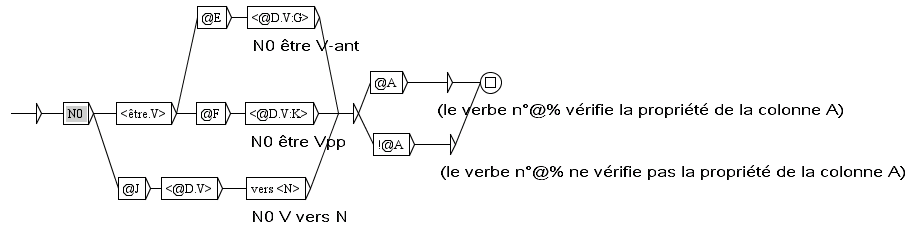
\includegraphics[width=15cm]{resources/img/fig8-3.png}
\caption{Exemple de graphe paramétré\label{fig-reference-graph}}
\end{center}
\end{figure}

\begin{figure}[!ht]
\begin{center}
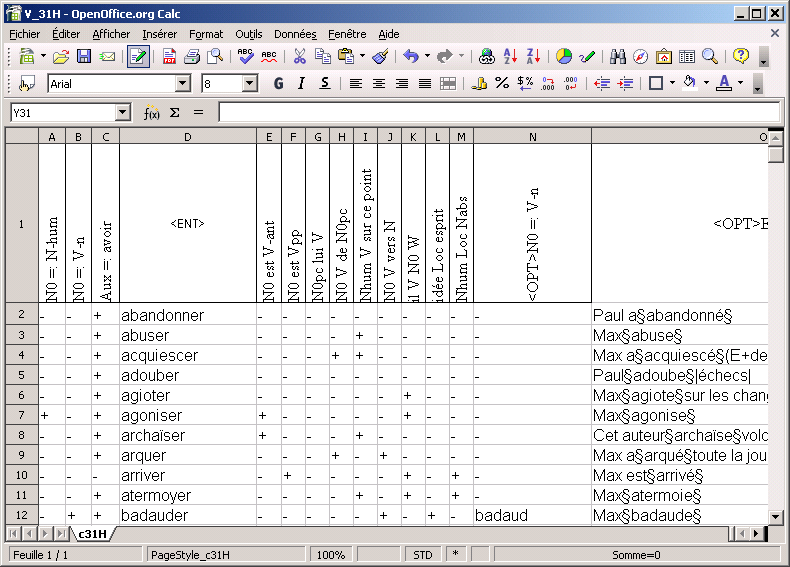
\includegraphics[width=15cm]{resources/img/fig8-4.png}
\caption{Table de lexique-grammaire 31H\label{fig-table-31H}}
\end{center}
\end{figure}


\subsection{Génération automatique de graphes}
Pour pouvoir générer des graphes à partir d’un graphe paramétré et d’une table, il faut
tout d’abord ouvrir la table en cliquant sur "Open..." dans le menu "Lexicon-Grammar" (voir
figure~\ref{fig-lexicon-grammar-menu}). La table doit avoir été préalablement convertie en texte
Unicode.

\begin{figure}[!ht]
\begin{center}
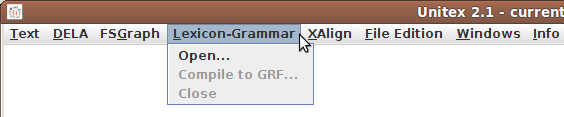
\includegraphics[width=12cm]{resources/img/fig8-5.png}
\caption{Menu "Lexicon-Grammar"\label{fig-lexicon-grammar-menu}}
\end{center}
\end{figure}

\bigskip
\noindent La table sélectionnée est alors affichée dans une fenêtre (voir
figure~\ref{fig-table-display}). Si elle n'apparaît pas sur l'écran, elle peut être occultée par
d'autres fenêtres Unitex.

\begin{figure}[!ht]
\begin{center}
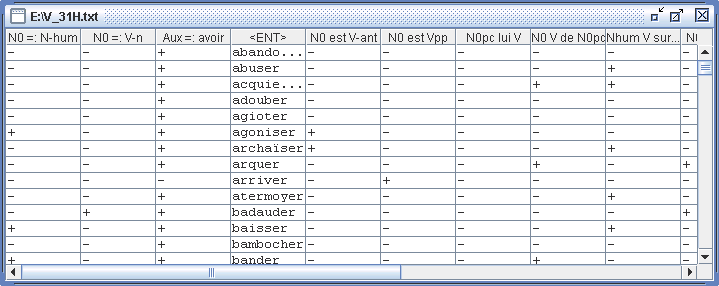
\includegraphics[width=15cm]{resources/img/fig8-6.png}
\caption{Displaying a table\label{fig-table-display}}
\end{center}
\end{figure}

\bigskip
\noindent  Pour générer automatiquement des graphes à partir d’un graphe paramétré, cliquez sur
"Compile to GRF..." dans le menu "Lexicon-Grammar". La fenêtre de la figure
\ref{fig-configuration-graph-generation} apparaît alors.


\begin{figure}[!ht]
\begin{center}
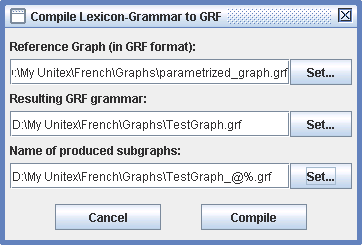
\includegraphics[width=9cm]{resources/img/fig8-7.png}
\caption{Configuration de la génération automatique de graphes\label{fig-configuration-graph-generation}}
\end{center}
\end{figure}

\bigskip
\noindent Dans le cadre "Reference Graph (in GRF format)", indiquez le nom du graphe paramétré
à utiliser. Dans le cadre "Resulting GRF grammar", indiquez le nom du graphe principal qui
sera généré. Ce graphe principal est un graphe faisant appel à tous les graphes qui auront
été générés. En lançant une recherche dans un texte avec ce graphe, vous appliquerez ainsi
simultanément tous les graphes générés.


\bigskip
\noindent  Le cadre "Name of produced subgraphs" permet de préciser le nom des graphes qui seront
générés. Afin d’être certain que tous les graphes auront des noms distincts, il est conseillé
d’utiliser la variable \verb+@%+, cette variable sera remplacée pour chaque entrée par le numéro de
celle-ci, garantissant ainsi que tous les graphes auront un nom différent. Par exemple, si l’on
remplit ce cadre avec le nom "\verb+TestGraph.grf+" et si les sous-graphes sont nommés
"\verb+TestGraph_@%.grf+", le sous-graphe généré à partir de la 16{\ieme}    ligne sera nommé  
"\verb+TestGraph_0016.grf+".

\bigskip
\noindent Les figures \ref{fig-archaiser} et \ref{fig-badauder} montrent deux graphes générés
en appliquant le graphe paramétré de la figure~\ref{fig-reference-graph} à la table 31H.

\bigskip
\noindent La figure~\ref{fig-main-graph} montre le graphe principal obtenu.

\begin{figure}[!ht]
\begin{center}
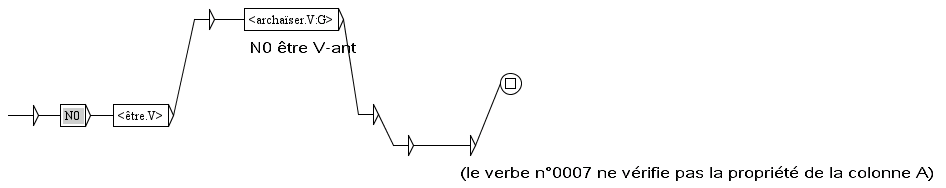
\includegraphics[width=15cm]{resources/img/fig8-8.png}
\caption{Graphe généré pour le verbe
\texttt{archa\"iser}\label{fig-archaiser}}
\end{center}
\end{figure}

\begin{figure}[!ht]
\begin{center}
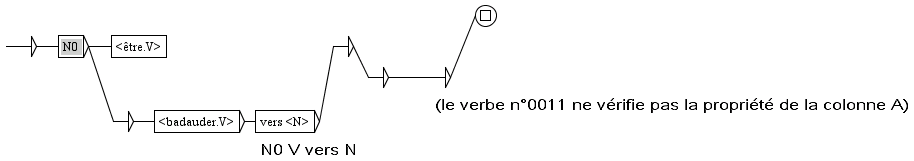
\includegraphics[width=15cm]{resources/img/fig8-9.png}
\caption{Graphe généré pour le verbe \texttt{badauder}\label{fig-badauder}}
\end{center}
\end{figure}

\begin{figure}[!ht]
\begin{center}
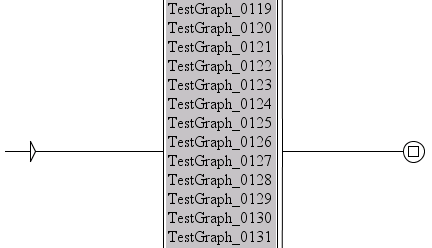
\includegraphics[width=10cm]{resources/img/fig8-10.png}
\caption{Graphe principal appelant tous les graphes générés\label{fig-main-graph}}
\end{center}
\end{figure}


